\documentclass[
  11pt, % The default document font size, options: 10pt, 11pt, 12pt
  codirector, % Uncomment to add a codirector to the title page
]{charter}
\usepackage{enumitem}
\usepackage{pdflscape}
\usepackage{tikz}
%\usetikzlibrary{shapes,arrows}
%\usepackage{tikz}
\usetikzlibrary{positioning, arrows.meta, backgrounds, fit}
\usepackage{fontawesome5}
\usepackage{tikz,tkz-tab}
\usepackage{booktabs} % Para tablas más elegantes
\usetikzlibrary{positioning, arrows.meta, backgrounds, fit}

\usetikzlibrary{matrix,arrows, positioning,shadows,shadings,backgrounds, calc, shapes, tikzmark}

\usepackage{fmtcount}
\usepackage{xurl}

\makeatletter
\newcommand{\mytwodigits}[1]{\two@digits{#1}}
\makeatother

\newcounter{reqCounter}
\setcounter{reqCounter}{0}


% Completar los siguintes Campos
\materia{Ingeniería de Software}
\bimestre{tercer bimestre}
\docentes{Alejandro Permingeat; Esteban	Volentini; Mariano Finochietto y Santiago Salamandri}
\titulo{Emulador de microprocesador Leon3 para desarrollo de software satelital y simuladores}
\posgrado{Carrera de Especialización en Sistemas Embebidos}
\autor{Ing. Iriarte Fernandez, Nicolás Ezequiel
  (NicolasIriarte95@gmail.com)}
\director{Esp. Lic. Horro, Nicolás Eduardo}
\pertenenciaDirector{INVAP.\@S.E.}
\codirector{}
\pertenenciaCoDirector{}
\cliente{Pinedo, Matías}
\empresaCliente{INVAP.\@SE}
\fechaINICIO{16 de noviembre de 2023}		%Fecha de entrega
\CODrequerimiento{NEMU-SR-}


\begin{document}

\maketitle
\tableofcontents

\newpage

\section*{Registros de cambios}
\label{sec:registro}


\begin{table}[ht]
	\label{tab:registro}
	\centering
	\begin{tabularx}{\linewidth}{@{}|c|X|c|@{}}
		\hline
		\rowcolor[HTML]{C0C0C0}
		Revisión & \multicolumn{1}{c|}{\cellcolor[HTML]{C0C0C0}Detalles de los cambios realizados} & Fecha      \\ \hline
		0      & Creación del documento.                                 &\fechaInicioName \\ \hline

    		1      & Se aplican cambios sugeridos por Salamandri Santiago. & 20 de noviembre de 2023 \\ \hline


    \hline

	\end{tabularx}
	\label{sec:cierre}
\end{table}

\pagebreak


\section{Introducción}
\label{sec:org60390fa}

%En esta sección se proporcionará una introducción a todo el documento de Especificación de Requisitos Software(ERS). Consta de varias subsecciones: propósito, ámbito del sistema, definiciones, referencias y visión general del documento.


\subsection{Propósito}
\label{sec:org434c3ef}

%En esta subsección se definirá el propósito del documento ERS y se especificará a quien va dirigido.

\begin{enumerate}
\item Este documento representa una especificación de requerimientos de software para un \textit{Emulador de microprocesador Leon3 para desarrollo de software satelital y simuladores}.

\item El presente documento está dirigido a:

  \begin{itemize}
  \item Desarrolladores de modelos simulados, quienes se encargan de desarrollar dispositivos de manera simulada.  Tales como podrían ser memorias, FPGAs y/o periféricos.

  \item Desarrolladores de software de vuelo, quienes se encargan de desarrollar drivers o software que usa interfaces de bajo nivel.

  \item Ingenieros de pruebas, quienes se encarga de automatizar los    ensayos de calificación de hardware y/o de componentes que lo emulen.
  \end{itemize}

\end{enumerate}


\subsection{Ámbito del sistema}
\label{sec:org12e44a1}

\begin{enumerate}
\item El software es el sistema a desarrollar como trabajo final de la Carrera de Especialización en Sistemas Embebidos.
\item El software será distribuido como una bibilioteca de Linux junto con una API para interactuar con la misma.
\item La API provista será en lenguaje C.
\item El software no incluirá emulación completa sobre todos los periféricos del microprocesador Leon3.
\end{enumerate}


\subsection{Definiciones, Acrónimos y Abreviaturas}
\label{sec:orgb158e36}

\begin{enumerate}
\item API: Application Programming Interface (interfaz de programación de aplicaciones).
\item CSV: Comma Separated Value.
\item FSW: Software de vuelo (Fly Software).
\item HW: Hardware.
\item N/A: Not Applicable (no aplicable).
\item SW: Software.
\end{enumerate}

\subsection{Referencias}
\label{sec:org62711e0}

\begin{enumerate}
\item \href{https://github.com/NicolasIriarte/Plan-proyecto-final/blob/main/IriarteNicolas.pdf}{Plan de proyecto del trabajo final}.


  \url{https://github.com/NicolasIriarte/Plan-proyecto-final/blob/main/IriarteNicolas.pdf}

\item \href{https://www.gaisler.com/index.php/products/processors/leon3}{FRONTGRADE GAISLER}.

\url{https://www.gaisler.com/index.php/products/processors/leon3}


\item \href{https://en.wikipedia.org/wiki/Emulator}{Emuladores}.

\url{https://en.wikipedia.org/wiki/Emulator}

\item \href{https://ubuntu.com/}{Ubuntu}.

\url{https://ubuntu.com/}

\end{enumerate}

\section{Descripción general}
\label{sec:orgc1c4017}

\subsection{Visión general del documento}
\label{sec:orgdaca22c}

Este documento se realiza siguiendo el estándar IEEE Std. 830-1998.


\subsection{Perspectiva del producto}
\label{sec:org24980a8}

\begin{enumerate}
\item El software a realizar deberá replicar el comportamiento del microprocesador Leon3, descrito en la figura \ref{fig:Components}. Siendo el circulo rojo el objeto de desarrollo principal.
\item El software a implementar deberá estár pensado para correr sobre ambientes Linux, y deberá proveer herramientas para la depuración de errores.
\end{enumerate}

\begin{figure}[htpb]
  \label{fig:Components}
  \centering
  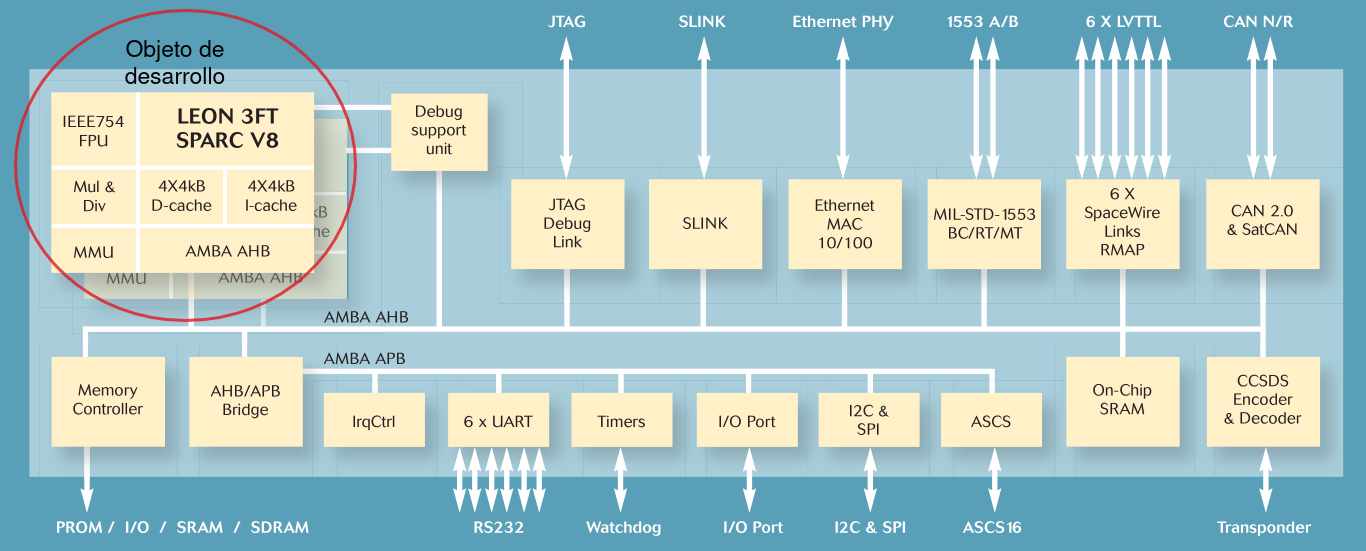
\includegraphics[width=1\textwidth]{./Figuras/Components.png}
  \caption{Diagrama en bloques del sistema.}
\end{figure}

\vspace{25px}


\subsection{Funciones del producto}
\label{sec:orgaf51da6}

\begin{enumerate}
\item El software aquí especificado brindará las siguientes funcionalidades:
  \begin{enumerate}
  \item Capacidad de carga y ejecución de SW de vuelo.
  \item Herramientas de depuración para inspeccionar y volcar registros y memorias emuladas.
  \item Emulación de un subset de instrucciones del microprocesador Leon3.
  \end{enumerate}
\item El software no incluirá las siguientes funcionalidades:
  \begin{enumerate}
  \item Emulación de todos los periféricos.
  \item Emulación de FPGAs.
  \end{enumerate}

\end{enumerate}



\subsection{Características de los usuarios}
\label{sec:orga40b0ee}

\begin{enumerate}
\item Los usuarios de dicho producto serán profesionales e interesados en su uso para ambientes simulados:
  \begin{itemize}
  \item Desarrolladores de software de vuelo.
  \item Desarrolladores de modelos simulados.
  \item Operadores satelitales.
  \end{itemize}
\item Dependiendo de su uso, los usuarios podrán tener conocimientos técnicos del hardware e interfaces emuladas o no.
\end{enumerate}

\subsection{Restricciones}
\label{sec:org5ca5790}

\begin{enumerate}
\item El software deberá estár bajo versiones controladas en Gitlab.
\item La API expuesta deberá estár contener documentación en código con Doxygen.
\item La API expuesta deberá ser en el lenguaje C.
\end{enumerate}

\subsection{Suposiciones y dependencias}
\label{sec:org0ae23fe}

\begin{enumerate}
\item Se tendrá acceso a un modelo de referencia, el cual podrá ser un procesador fisico o emulado para realizar pruebas y/o comparaciones.
\item Se tendrá contacto directo con expertos para realizar consultas sobre el funcionamiento del microprocesador.
\end{enumerate}

\subsection{Requisitos futuros}
\label{sec:org33cfcdb}

N/A.


\section{Requisitos específicos}
\label{sec:org40573d1}



\subsection{Interfaces externas}
\label{sec:orgfd5391f}

\begin{description}

\item[\textbf{[\CODrequerimiento\mytwodigits{\value{reqCounter}}]}]: El software deberá exponer una API en el lenguaje C.
  \stepcounter{reqCounter}

\item[\textbf{[\CODrequerimiento\mytwodigits{\value{reqCounter}}]}]: El software deberá proveer acceso a los registros del procesador emulado.
  \stepcounter{reqCounter}

\item[\textbf{[\CODrequerimiento\mytwodigits{\value{reqCounter}}]}]:  El software deberá poder inspeccionar y volcar memorias emuladas.
  \stepcounter{reqCounter}


\end{description}



\subsection{Funciones}
\label{sec:org307bb59}

\begin{description}

\item[\textbf{[\CODrequerimiento\mytwodigits{\value{reqCounter}}]}]: El software deberá poder cargar los mismos binarios que el microprocesador fisico.
  \stepcounter{reqCounter}

\item[\textbf{[\CODrequerimiento\mytwodigits{\value{reqCounter}}]}]: El software deberá emular el microprocesador en cada ciclo de reloj.
  \stepcounter{reqCounter}

\item[\textbf{[\CODrequerimiento\mytwodigits{\value{reqCounter}}]}]: El software deberá exponer y emular un mapa de memoria donde otros dispositivos, ajenos a este proyecto, podrán leer y escribir.
  \stepcounter{reqCounter}

\item[\textbf{[\CODrequerimiento\mytwodigits{\value{reqCounter}}]}]: El software deberá emular las instrucciones de lectura y escritura de memoria.
  \stepcounter{reqCounter}

\item[\textbf{[\CODrequerimiento\mytwodigits{\value{reqCounter}}]}]: El software deberá emular las instrucciones de suma, resta y multiplicación.
  \stepcounter{reqCounter}

\item[\textbf{[\CODrequerimiento\mytwodigits{\value{reqCounter}}]}]: El software deberá emular las de instrucciones de salto condicionales, tales como operaciones \textit{if} y \textit{jumps}.
  \stepcounter{reqCounter}

\item[\textbf{[\CODrequerimiento\mytwodigits{\value{reqCounter}}]}]: El software deberá permitir pausas en la ejecución para inspeccionar y volcar registros y memorias emuladas.
  \stepcounter{reqCounter}

\item[\textbf{[\CODrequerimiento\mytwodigits{\value{reqCounter}}]}]: El software deberá permitir la ejecución de instrucciones paso a paso.
  \stepcounter{reqCounter}

\item[\textbf{[\CODrequerimiento\mytwodigits{\value{reqCounter}}]}]: El software deberá permitir la ejecución de instrucciones en modo continuo.
  \stepcounter{reqCounter}

\end{description}


\subsection{Requisitos de rendimiento}
\label{sec:org94bc543}

\begin{description}

\item[\textbf{[\CODrequerimiento\mytwodigits{\value{reqCounter}}]}]: El software deberá ejecutar instrucciones en tiempo real (Ejecución a 1X).
  \stepcounter{reqCounter}

\end{description}


\subsection{Restricciones de diseño}
\label{sec:org49fe900}

\begin{description}

\item[\textbf{[\CODrequerimiento\mytwodigits{\value{reqCounter}}]}]: El software deberá poder compartirse sin necesidad de exponer el código fuente del mismo.
  \stepcounter{reqCounter}

\end{description}


\subsection{Atributos del sistema}
\label{sec:orgd0babc0}

N/A.

\subsection{Otros requisitos}
\label{sec:org31d2978}

\begin{description}

\item[\textbf{[\CODrequerimiento\mytwodigits{\value{reqCounter}}]}]: El software deberá poder ejecutarse sobre Ubuntu 22.04 LTS.
  \stepcounter{reqCounter}


\item[\textbf{[\CODrequerimiento\mytwodigits{\value{reqCounter}}]}]: El software deberá poder ejecutarse en multiples instancias simultaneamente.
  \stepcounter{reqCounter}

\item[\textbf{[\CODrequerimiento\mytwodigits{\value{reqCounter}}]}]: El software deberá estár acompañado de un manual de usuario en formato PDF.
  \stepcounter{reqCounter}

\item[\textbf{[\CODrequerimiento\mytwodigits{\value{reqCounter}}]}]: El software deberá estár acompañado de documentación de referencia en formato web (Exportación de Doxygen a HTML).
  \stepcounter{reqCounter}


\end{description}

\end{document}
